\subsection{All About Parallel Transmission Line Matching!}

\begin{tcolorbox}[colback=gray!10, colframe=black, title=E9E03] 

What matching system uses a short length of transmission line connected in parallel with the feed line at or near the feed point?

\begin{enumerate}[label=\Alph*.]
    \item Gamma match
    \item Delta match
    \item T-match
    \item \textbf{Stub match}
\end{enumerate} \end{tcolorbox}

\subsubsection{Related Concepts}

The concept of impedance matching is crucial in radio communication and electronics, particularly when dealing with antennas and transmission lines. The goal of impedance matching is to ensure maximum power transfer from the source to the load, which, in this case, is typically an antenna. When the impedances are mismatched, reflections occur, resulting in standing waves that can cause signal loss.

One of the methods for achieving this matching is through the use of a stub match. A stub match involves the addition of a short length of transmission line, known as a stub, which is connected in parallel with the main feed line at or near the feed point of the antenna. This stub can be either open-circuited or short-circuited, and its length and characteristics can be adjusted to alter the impedance seen by the feed line, thus achieving the desired match.

\subsubsection{Mathematical Considerations}

To analyze a stub match, one might use the transmission line equations. Typically, for a given transmission line with characteristic impedance \( Z_0 \), and a load impedance \( Z_L \), the input impedance \( Z_{in} \) can be expressed using the following formula:

\[
Z_{in} = Z_0 \frac{Z_L + j Z_0 \tan(\beta l)}{Z_0 + j Z_L \tan(\beta l)}
\]

Where:
- \( \beta \) is the phase constant,
- \( l \) is the length of the stub.

To achieve matching, the input impedance \( Z_{in} \) must equal the desired system impedance (commonly 50 ohms in RF systems).

\subsubsection{Diagram}

A diagram illustrating the configuration of a stub match can be beneficial to understand its operation. The following code snippet creates a simple diagram using TikZ:

\begin{center}
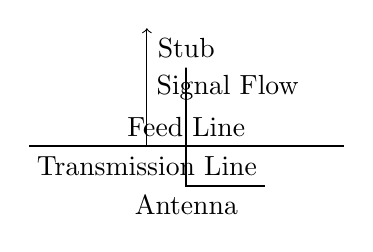
\begin{tikzpicture}[scale=1]
    \draw[thick] (0,0) -- (4,0) node[midway, above] {Feed Line};
    \draw[thick] (2,0) -- (2,1) node[above] {Stub} -- (2,0.5) -- (2,0);
    \draw[thick] (2,0) -- (2,-0.5) node[below] {Antenna} -- (3,-0.5);
    \draw[dashed] (2,0) -- (1,0) node[midway, below] {Transmission Line};
    \draw[->] (1.5,0) -- (1.5,1.5) node[midway,right] {Signal Flow};
\end{tikzpicture}
\end{center}
